\chapter{Analiza problemu}
\thispagestyle{chapterBeginStyle}
\label{rozdzial1}

Rozdział ten poświęcony jest analizie problemu i próbą przedstawienia go świecie wirtualnym. Szczegółowe algorytmy oraz wzory znajdują się w rozdziale 3. w podpunkcie traktującym o module opisującym model.

\section{Budowa łamigłówki}

Model składa się z mniejszych sześciennych elementów połączonych ze sobą w sposób umożliwiający obracanie poszczególnych kostek względem siebie.

\begin{figure}[h]
    \centering
    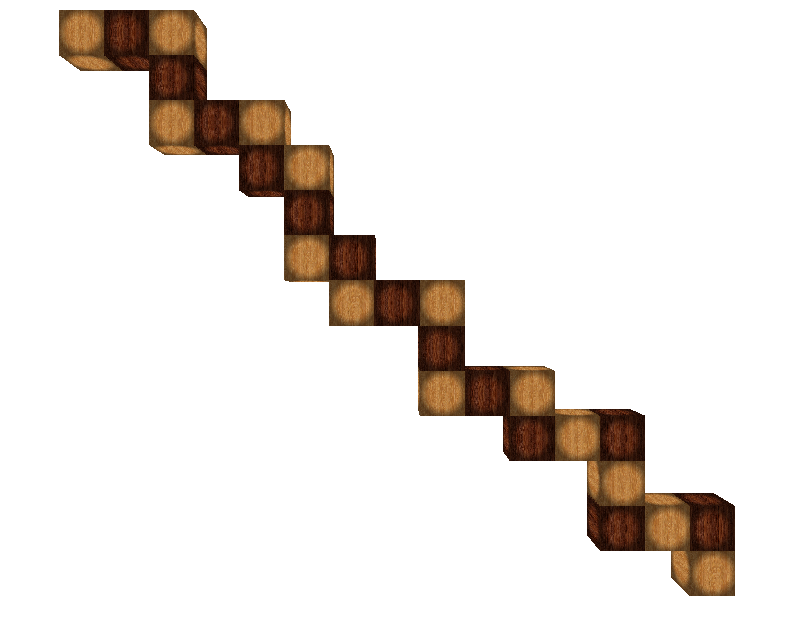
\includegraphics[width=0.7\textwidth]{start}
    \caption{Na zdjęciu widoczny ciąg połączonych ze sobą sześcianów – model w fazie początkowej.}
    \label{fig:joints1}
\end{figure}

\section{Przedstawienie łamigłówki w pamięci komputera}

Model zagadki konstruowany jest po dostarczeniu wektora długości poszczególnych fragmentów do aplikacji. Mniejsze sześciany umieszczane są w przestrzeni trójwymiarowej przez algorytm analizujący.

Między każdym łączeniem możliwy jest ruch rotacyjny, lecz nie każdy ruch jest znaczący dla stanu całego model. Wykonywanie ruchów w łączeniach nieznaczących jest redundantne, tj. uzyskanie stanu modelu po każdym możliwym obrocie w łączeniu nieznaczącym jest możliwe po wykonaniu ruchu na jednym z najbliższych łączeń znaczących. Przez analiza pokryte jest również wykrywanie połączeń znaczących.

\section{Cel zagadki}

Na podstawie wektora wejściowego obliczany jest najmniejszy bok sześcianu, w którym możliwe jest umieszczenie złożonego modelu. 
